% ===========================================
% IN-CIRCUIT SERIAL PROGRAMMING GUIDE
% Written by: Braidan Duffy
%
% Date: 05/22/2022
% Last Revision: 05/24/2022
% ============================================

\pagelayout{wide} % Remove margins
\chapter{In-Circuit Serial Programming Guide}

Microcontrollers are special embedded processors that are capable of executing specific code with a high efficiency.
They are used throughout the world in various devices ranging from handheld gaming devices, medical units, military 
hardware, and digital signage. Recently, the Arduino foundation made playing with microcontrollers easier as they
created a platform where users could write code, plug in a microcontroller over USB, flash the chip, and see the results
- nearly in real-time. They helped usher in the Maker Renaissance we found ourselves in today, by obfuscating the more
complex tasks in microcontroller programming using high-level software and other microcontrollers.

The purpose of this guide is to help de-obfuscate low-level microcontroller programming by showing you what is really happening when you give the "Upload" command in the Arduino IDE.

\section*{What is In-Circuit Serial Programming?}

In-Circuit Serial Programming (ICSP) is the fundamental way to program a microcontroller. Microcontrollers typically
store their programs on SPI flash memory which can be read or written over as the programmer demands. By temporarily 
disabling the microcontroller and overwriting the contents of the SPI flash memory, we can reprogram the microcontroller
with different code.

On the Arduino boards, when you upload code over USB, a secondary microcontroller on the board interprets the USB
communications and translates them to the UART serial protocol. The bootloader on the main microcontroller then uses 
the data coming from the UART bus to reprogram the SPI flash memory, thus reprogramming the Arduino. This is a form of 
ICSP, but adds complexity to both the circuit and fundamental microcontroller firmware. 

A simpler version of ICSP is accessing the SPI flash memory directly. On the Arduino Uno board, the ICSP header is 
easily visible and can be used by any device that has an SPI bus to reprogram the microcontroller. 
If, for instance, the USB-Serial bridge on the board has its program memory corrupted ICSP can be used to re-flash the 
correct firmware onto the chip. Alternatively, if the chip is completely non-functional, the primary microcontroller 
can still be used with new code being deployed over the ICSP pins.

\begin{figure}
    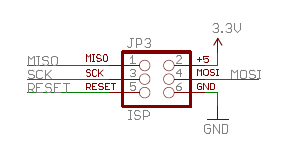
\includegraphics[width=3.5in]{rpi_icsp/icsp-header.png}
    \caption[Arduino ICSP Header]{Pinout of the Arduino Uno and Mega ICSP header}
    \labfig{arduino_icsp_header}
\end{figure}

Note that different microcontrollers may have different implementations of ICSP. Another popular form is the Single
Wire interface. Please refer to your microcontroller's datasheet for specific information.

\section*{Arduino as In-circuit Serial Programmer}

For this example, we will be using an Arduino as an In-circuit Serial Programmer (ISP) to program another Arduino over 
ICSP. The Arduino Foundation provides a sketch in the examples folder of the Arduino IDE to configure an Arduino board 
as an ISP. First, plug in the Arduino Uno to the ICSP header as shown in Figure \ref{fig:arduino_icsp_hookup} and according to Table \ref{tab:arduino_icsp_hookup}. On most boards, there is no reverse-polarity protection, so make sure the 5V and GND wires are plugged in correctly. 

\begin{figure}
    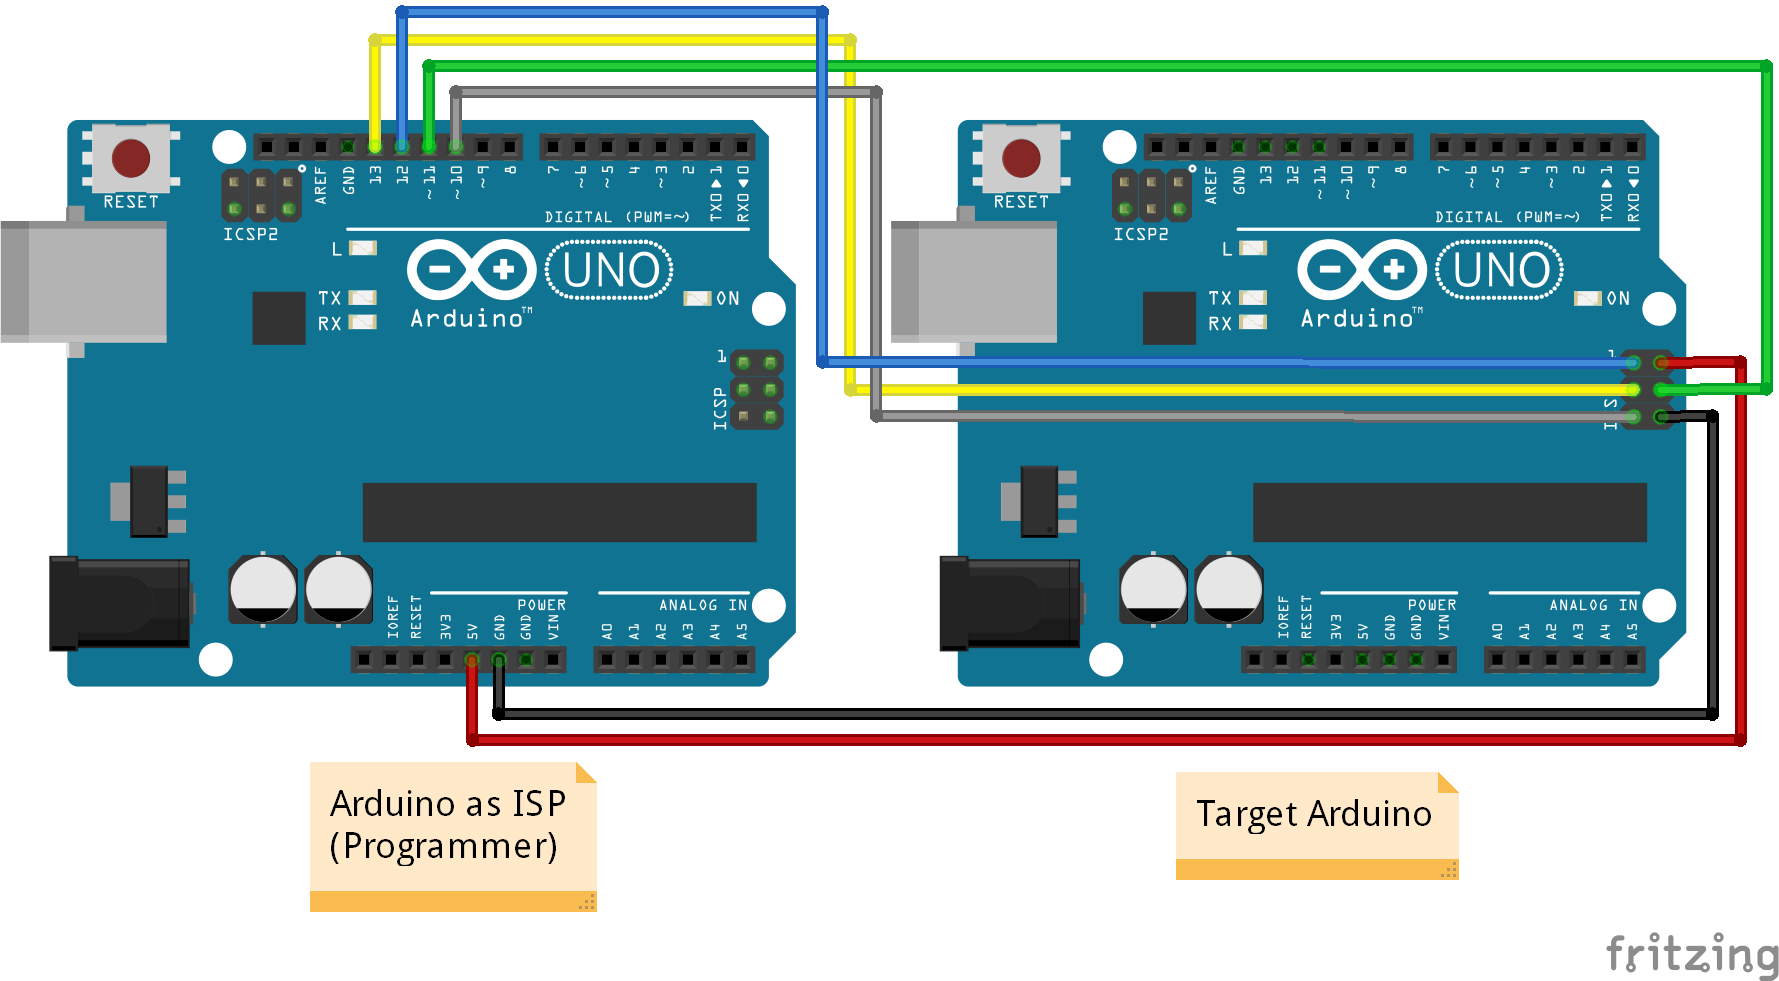
\includegraphics[]{rpi_icsp/Fritzing_ArduinoasISP_AVR_Programmer_bb.png}
    \caption[ArduinoISP Hookup Diagram]{Diagram showing how to hook up an ArduinoISP programmer and Arduino ICSP target.Retrieved from \url{https://learn.sparkfun.com/tutorials/installing-an-arduino-bootloader/hardware-hookup}}
    \labfig{arduino_icsp_hookup}
\end{figure}

\begin{table}[h!]
    \caption[ArduinoISP Hookup Guide]{ArduinoISP hookup table for target and programmer}
    \begin{tabular}{ c | c }
        \toprule
        Programmer & Target \\

        \midrule
        DIO 12  & MISO (Pin 1)  \\
        DIO 13  & SCK (Pin 2)   \\
        DIO 10  & RESET (Pin 3) \\
        5V      & 5V (Pin 4)    \\
        DIO 11  & MOSI (Pin 5)  \\
        GND     & GND (Pin 6)   \\

        \bottomrule
    \end{tabular}
    \labtab{arduino_icsp_hookup}
\end{table}

After wiring up the boards, plug the Arduino Uno into the programming computer. This will apply power to the system and should allow you to program the Uno as you normally would. Then, navigate the ArduinoISP sketch located in the “examples” folder of the Arduino IDE (Figure \ref{fig:arduino_isp_loc}) and upload the sketch to the Arduino Uno.

\begin{figure}
    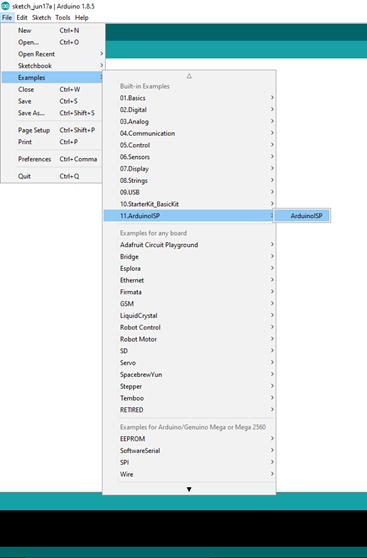
\includegraphics[width=3.5in]{rpi_icsp/ArduinoISP_ss.png}
    \caption[ArduinoISP Example]{Location of ArduinoISP sketch in the Arduino IDE}.
    \labfig{arduino_isp_loc}
\end{figure}

Once the ArduinoISP sketch is uploaded, navigate to a sketch to upload to the target board configuring the compiler to the target board and processor (Figure \ref{fig:arduino_isp_config}). 
Use the same COM port as the Arduino Uno and use the “Upload Using Programmer” option  shown in Figure \ref{fig:arduino_isp_upload}. 
If you get any errors such as “Unable to communicate with device” or “Invalid device signature”, check your wiring and try again.

\begin{figure}
    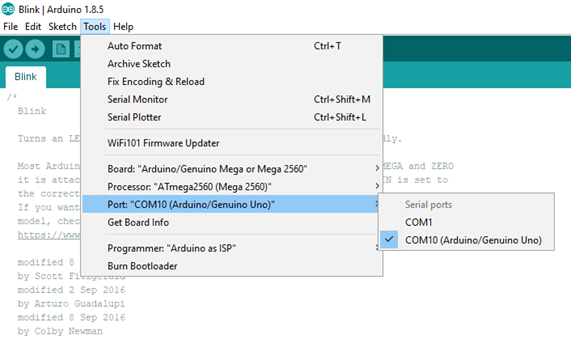
\includegraphics[width=6in]{rpi_icsp/ArduinoISP_config_ss.png}
    \caption[ArduinoISP Config]{Configuring the Arduino IDE to compile for the correct board}.
    \labfig{arduino_isp_config}
\end{figure}

\begin{figure}
    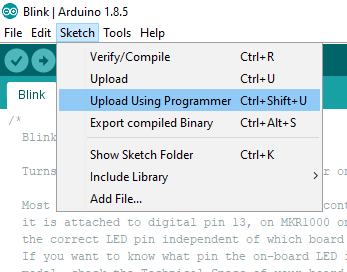
\includegraphics[width=3.5in]{rpi_icsp/ArduinoISP_upload_ss.png}
    \caption[ArduinoISP Upload]{Upload Using Programmer sketch option}.
    \labfig{arduino_isp_upload}
\end{figure}

While this example used the basic Blink example code, this process can be done for any appropriate Arduino sketch onto most Arduino-compatible boards. 
On some embedded devices, a common USB interface may not be accessible and therefore ICSP is the only programming option.

\section*{Using a Raspberry Pi as ISP}

For the graduate portion of this class, we will be using a Raspberry Pi to upload code to the Arduino boards over ICSP. 
The Raspberry Pi uses 3.3V logic levels which are not completely compatible with the 5V logic levels of the Arduino board.
Therefore, it is strongly recommended to use a breadboard to breakout the Raspberry Pi's pins to a logic level converter
and connect it from there to the Arduino's ICSP header. Please refer to Figure \ref{fig:rpi_icsp_bb} for hookup information. 
The pinout for this configuration can be found in the figure, which we will use later with AVRDUDE

    \begin{figure}[h!]
        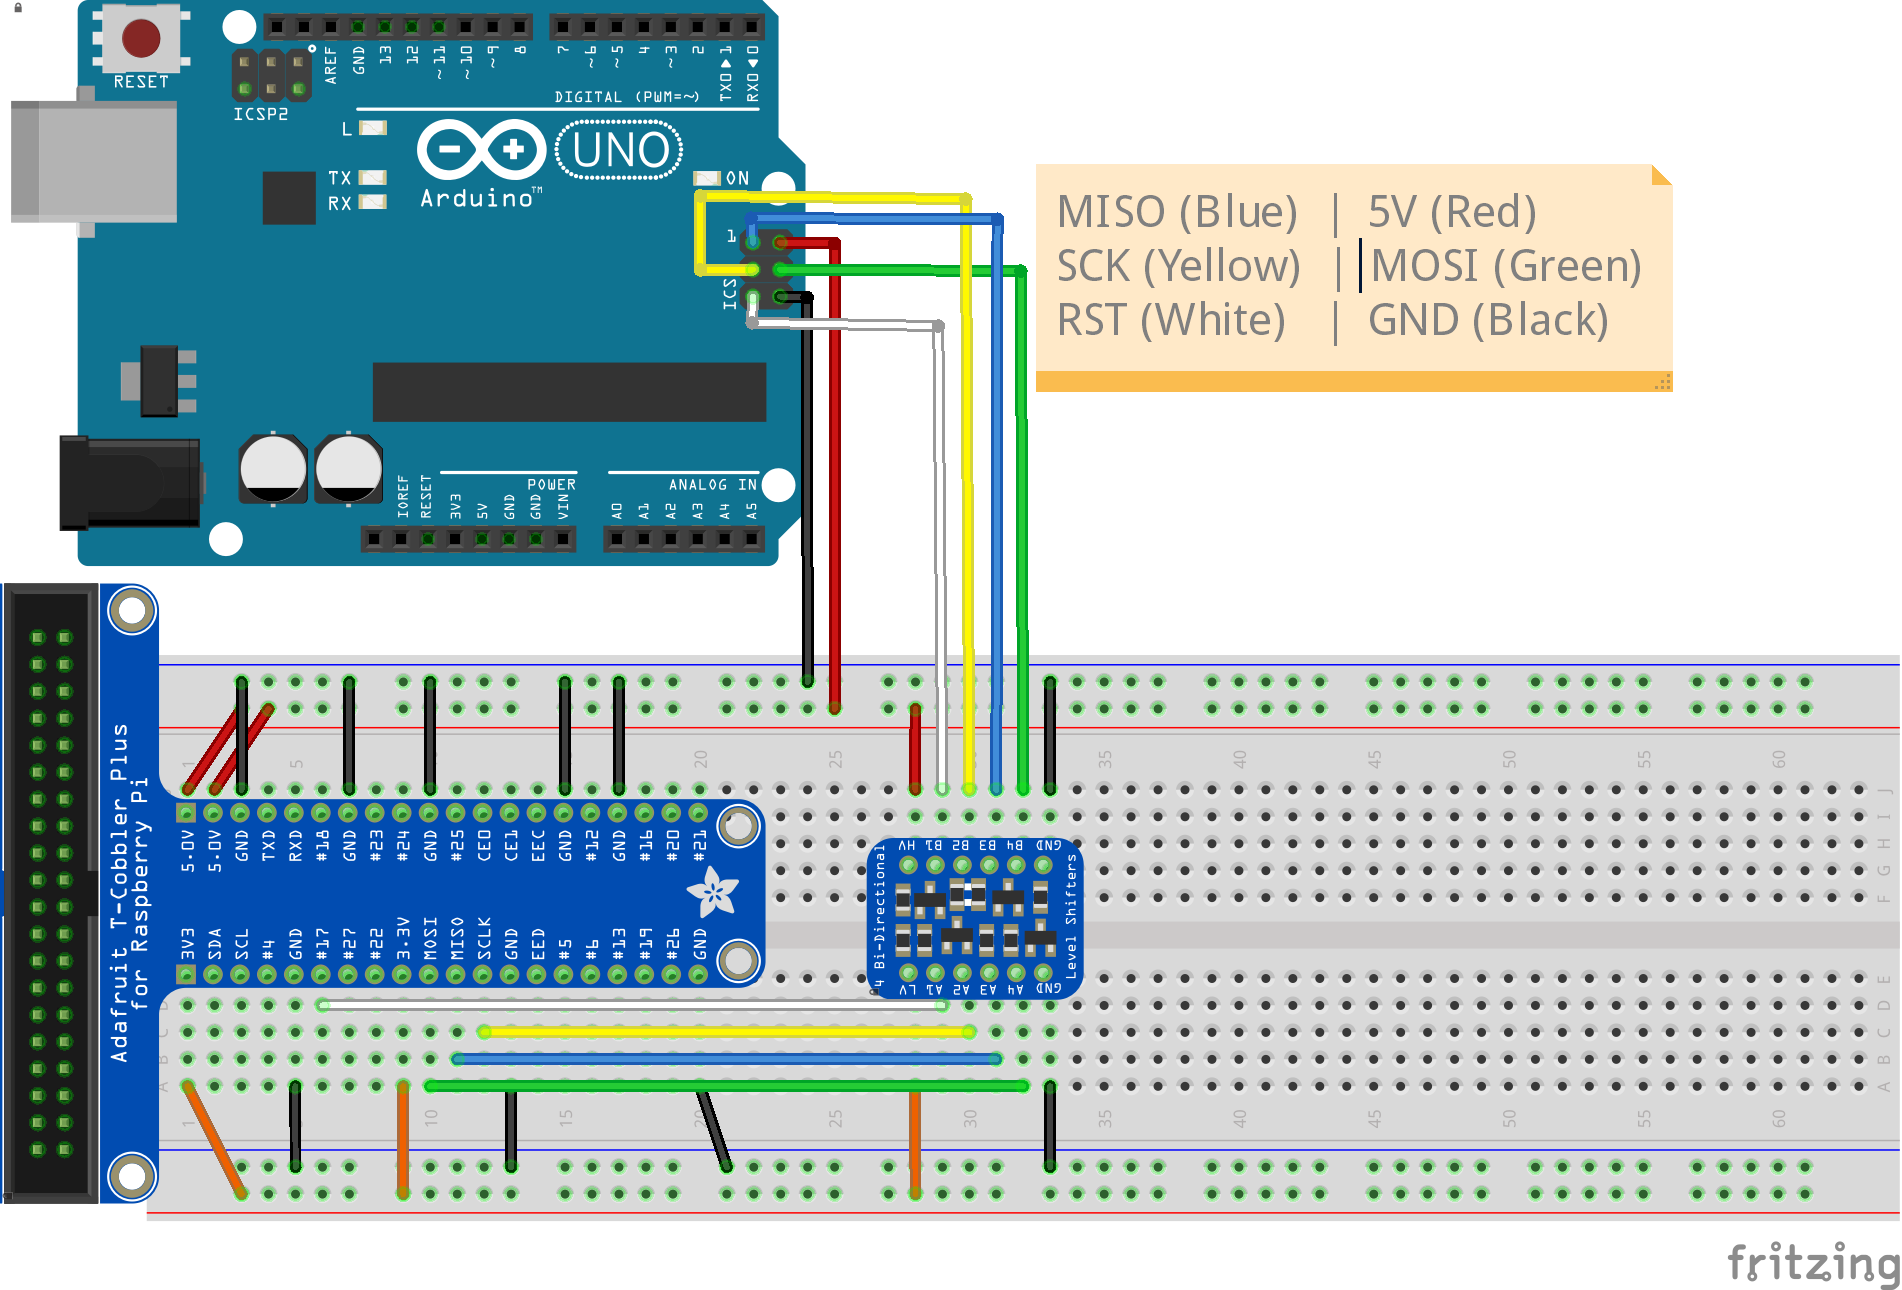
\includegraphics[width=5in]{rpi_icsp/rpi_icsp_bb.png}
        \caption[Raspberry Pi ISP Breadboard]{A wiring diagram of how the Raspberry Pi should be connected to the Arduino ICSP headers through a breadboard and a \href{https://www.adafruit.com/product/757}{logic-level     converter}. 
        Created using Fritzing \url{https://fritzing.org}}.
        \labfig{rpi_icsp_bb}
    \end{figure}

    \begin{table}[h!]
        \caption[RaspberryPi as ISP Hookup Guide]{Raspberry Pi as ISP hookup table for target and programmer}
        \begin{tabular}{ l | c | c }
            \toprule
            Programmer & Logic Level Converter & Target \\
    
            \midrule
            3V3                                 & LV    & NC\footnotemark   \\
            NC\footnotemark[\value{footnote}]   & HV    & 5V                \\
            GPIO 17                             & A1/B1 & RESET             \\
            GPIO 11 (SCLK)                      & A2/B2 & SCK               \\
            GPIO 9 (MISO)                       & A3/B3 & MISO              \\
            GPIO 10 (MOSI)                      & A4/B4 & MOSI              \\
            GND                                 & GND   & GND               \\
    
            \bottomrule
        \end{tabular}
        \labtab{rpi_icsp_hookup}
    \end{table}
    \footnotetext{Not connected}

    \subsection*{Setting up AVRDUDE}
    AVRDUDE is the software package that will upload machine binary to the microcontroller's program storage. 
    The following steps will assume you have already set up the Raspberry Pi with RaspberryPiOS and updated the latest packages. 
    Through this example, we will be operating inside a command terminal through a remote secure login shell, but this process can be repeated inside the command terminal of a headed set up.

    First, in the open terminal execute the following command:

    \begin{lstlisting}[style=kaolstplain,linewidth=1.5\textwidth]
    sudo apt-get install avrdude
    \end{lstlisting}

    This will install AVRDUDE on the Raspberry Pi so we can flash .hex files onto the microcontroller. To verify the installation, execute:

    \begin{lstlisting}[style=kaolstplain,linewidth=1.5\textwidth]
    avrdude -v
    \end{lstlisting}

    If the output is something like:

    \begin{lstlisting}[style=kaolstplain,linewidth=1.5\textwidth]
    avrdude: Version 6.3-20171130
        Copyright (c) 2000-2005 Brian Dean, http://www.bdmicro.com/
        Copyright (c) 2007-2014 Joerg Wunsch

        System wide configuration file is "/etc/avrdude.conf"
        User configuration file is "/home/pi/.avrduderc"
        User configuration file does not exist or is not a regular file, skipping

    avrdude: no programmer has been specified on the command line or the config file
        Specify a programmer using the -c option and try again
    \end{lstlisting}

    Then the installation is good and AVRDUDE has created a user configuration file that we can edit. To begin this process, execute the following commands in the terminal:

    \begin{lstlisting}[style=kaolstplain,linewidth=1.5\textwidth]
    cp /etc/avrdude.conf ~/avrdude_gpio.conf
    \end{lstlisting}

    \begin{lstlisting}[style=kaolstplain,linewidth=1.5\textwidth]
    nano ~/avrdude_gpio.conf
    \end{lstlisting}

    The first command copies the default AVRDUDE configuration file to a new file in the home directory of user. 
    The second command will open this file in the Nano file editor, pulling up a screen like Figure \ref{fig:avrdude_gpio_config_nano}.
    
    \begin{figure}[h!]
        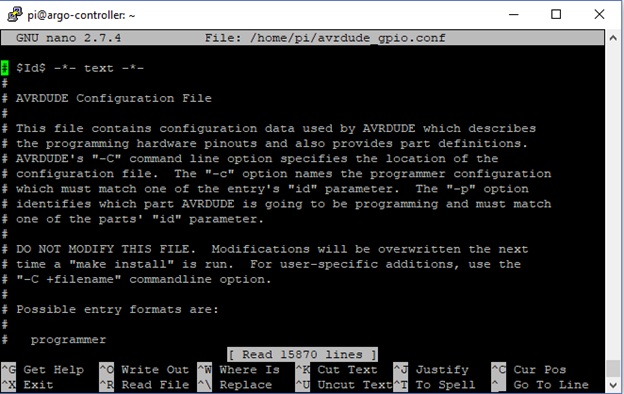
\includegraphics[]{rpi_icsp/avrdude_gpio_conf_nano_ss.png}
        \caption[AVRDUDE GPIO config file open in Nano]{The top of the avrdude\_gpio.conf file in Nano}
        \labfig{avrdude_gpio_config_nano}
    \end{figure}

    Once in the file, press CTRL\+\_, then CTRL\+V to navigate to the bottom of the file. There, paste the following block of code:

    \begin{lstlisting}[style=kaolstplain,linewidth=1.5\textwidth]
    programmer
        id = "gpio_icsp";
        desc = "Use the Linux sysfs interface to bitbang GPIO lines for programming the Arduino;
        type = "linuxgpio";
        reset = 17;
        sck = 11;
        mosi = 10;
        miso = 9;
    ;
    \end{lstlisting}

    This creates an AVRDUDE programmer that uses the GPIO pins specified in Table \ref{tab:rpi_icsp_hookup} to program the Arduino over ICSP. Press CTRL+X then Y then ENTER to save and exit the file; the AVRDUDE programming tool is now configured.

    \subsection*{Preparing a Sketch for ICSP Uploading (Arduino)}

    Once you have a sketch ready for the microcontroller to run, configure the compiler for your board, same as Figure \ref{fig:arduino_isp_config}.
    Select the ``Export compiled Binary'' option in the Arduino IDE (Figure \ref{fig:arduino_ide_export}). 
    This will create two files in the sketch`s directory, both ending with ``.hex'', but one will have ``.with\_bootloader'' in the middle. 
    The file we want to upload is the one without the bootloader, highlighted in Figure \ref{fig:arduino_sketch_folder}. \footnotemark
    
    \footnotetext{This will disable the USB programming bootloader. This will need to be re-flashed with the bootloader if you want to upload code to the microcontroller via USB again.}
    
    \begin{figure}[h!]
        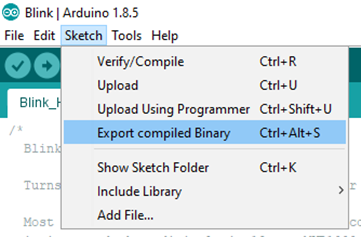
\includegraphics[width=3.5in]{rpi_icsp/arduino_export_binary_ss.png}
        \caption{Arduino IDE ``Export compiled Binary'' option}
        \labfig{arduino_ide_export}
    \end{figure}

    \begin{figure}[h!]
        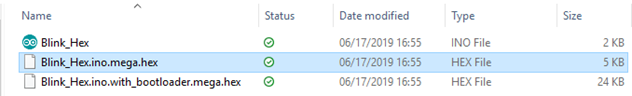
\includegraphics[]{rpi_icsp/arduino_binary_folder_ss.png}
        \caption{The sketch and its compiled binaries in their folder}
        \labfig{arduino_sketch_folder}
    \end{figure}

    \subsection*{Preparing a Sketch for ICSP Uploading (VS Code)}

    This part assumes you have already initialized the Arduino development environment within VS Code.
    In VS Code, open the ``arduino.json'' file in the /.vscode folder of your workspace. Add the following line to the bottom of the file:

    \begin{lstlisting}[style=kaolstplain,linewidth=1.5\textwidth]
    "output": ".arduinobuild"
    \end{lstlisting}

    This will create a new folder in the root directory of the workspace called ``.arduinobuild'' that will hold all of pre-compiled binaries for your Arduino sketch, logs, and other things that are not important right now.
    Inside this folder will be two files: ``[sketch\_name].ino.bin'' and ``[sketch\_name].bootloader.bin''.
    As before, the one we want to upload is the one without the bootloader.\footnotemark[1]

    \subsection*{Programming the Microcontroller}

    Transfer the binary file to the Raspberry Pi using your preferred method of choice.
    This is most easily done over a USB stick or a File Transfer Protocol like Secure Copy.
    Applications like \href{https://winscp.net/eng/download.php}{WinSCP} make this process easy for beginners.
    Place the file in a working destination directory - ideally, a project folder you have already set up beforehand.
    Then, open a terminal on the Raspberry Pi and execute the following command:
    
    \begin{lstlisting}[style=kaolstplain,linewidth=1.5\textwidth]
    sudo avrdude -p [Microcontroller] -C ~/avrdude_gpio.conf -c gpio_icsp -v
    \end{lstlisting}

    Note: the \textbf{[Microcontroller]} in this command needs to be replaced with the name of the microcontroller in use (e.g. ``atmega328p'' for the Arduino Uno or ``atmega2560'' for the Arduino Mega).

    This will verify that the Raspberry Pi can talk to the microcontroller and verifies that the chip is operating nominally.

    If there are any issues, make sure you are executing this command with ``sudo'' and that the configuration file matches with the GPIO pins used in the schematic; check the wiring connections to the Arduino; and check that the file path for ``avrdude\_gpio.conf'' is correct .\footnote{The "\textasciitilde" in the file path only denotes the relative directory you are currently in. If the file is NOT in the same directory that you are executing the command in, you must put the path in lieu of the “\textasciitilde ”.}

    Once you have established communications with the Arduino, execute:

    \begin{lstlisting}[style=kaolstplain,linewidth=1.5\textwidth]
    sudo avrdude -p [Microcontroller] -C ~/avrdude_gpio.conf -c gpio_icsp -v -U flash:w:[filename]:i
    \end{lstlisting}

    Where again \textbf{[Microcontroller]} needs to be replaced with the name of the microcontroller and \textbf{[filename]} needs to be replaced with the path and name of the binary sketch file you copied to the Raspberry Pi.
    The end of a successful write should look something like this:

    \begin{lstlisting}[style=kaolstplain,linewidth=1.5\textwidth]
    avrdude: AVR device initialized and ready to accept instructions

    Reading | ################################################## | 100% 0.00s

    avrdude: Device signature = 0x1e9801 (probably m2560)
    avrdude: safemode: lfuse reads as FF
    avrdude: safemode: hfuse reads as D8
    avrdude: safemode: efuse reads as FD
    avrdude: NOTE: "flash" memory has been specified, an erase cycle will be performed
            To disable this feature, specify the -D option.
    avrdude: erasing chip
    avrdude: reading input file "Blink_Hex.ino.mega.hex"
    avrdude: writing flash (1462 bytes):

    Writing | ################################################## | 100% 0.41s

    avrdude: 1462 bytes of flash written
    avrdude: verifying flash memory against Blink_Hex.ino.mega.hex:
    avrdude: load data flash data from input file Blink_Hex.ino.mega.hex:
    avrdude: input file Blink_Hex.ino.mega.hex contains 1462 bytes
    avrdude: reading on-chip flash data:

    Reading | ################################################## | 100% 0.82s

    avrdude: verifying ...
    avrdude: 1462 bytes of flash verified

    avrdude: safemode: lfuse reads as FF
    avrdude: safemode: hfuse reads as D8
    avrdude: safemode: efuse reads as FD
    avrdude: safemode: Fuses OK (E:FD, H:D8, L:FF)

    avrdude done.  Thank you.
    \end{lstlisting}

    If there is an error (most commonly with a file name) it will likely occur after the first reading block. 
    The -v argument of the command gives error statements in the output so you can error trace and find the problem. 
\pagelayout{margins} % Restore margins